\documentclass[12pt, french]{article}

\usepackage{fancyhdr, fancybox, lastpage}
\usepackage[most]{tcolorbox}
\usepackage[a4paper, margin={0.3in, .75in}]{geometry}
\usepackage{wrapfig}
\pagestyle{fancy}
\renewcommand\headrulewidth{1pt}
\renewcommand\footrulewidth{1pt}
\fancyhf{}
\rhead{ \em{Zakaria Haouzan}}
\lhead[C]{\em{1ére année baccalauréat Sciences Mathématiques}}
\chead[C]{}
\rfoot[C]{}
\lfoot[R]{}
\cfoot[]{\em{Page \thepage / \pageref{LastPage}}}


\newtcolorbox{Box2}[2][]{
                lower separated=false,
                colback=white,
colframe=white!20!black,fonttitle=\bfseries,
colbacktitle=white!30!gray,
coltitle=black,
enhanced,
attach boxed title to top left={yshift=-0.1in,xshift=0.15in},
title=#2,#1}


\begin{document}
\begin{center}
   \shadowbox {\bf{ ÉNERGIE POTENTIELLE DE PESANTEUR - ÉNERGIE MÉCANIQUE }}
\end{center}


%%_________________________Exercice ! :"_________________________Exercice
   \begin{Box2}{Exercice 1 : }
      Une balle de masse m = 200 g est lancé verticalement vers le haut avec une vitesse de valeur $5,0 m.s^{-1}$ à partir d'un point situé à 1,20 m du sol.

1. Calculer les énergies potentielle, cinétique et mécanique de la balle à l'état initial.

2. Calculer l'altitude maximale de la balle lors de ce lancer.

3. Calculer la vitesse de la balle au moment où elle retombe sur le sol.
      Donnée : $g = 9,8 N.kg^{-1}$ .
   \end{Box2}


%%_________________________Exercice !2 :"_________________________Exercice
\begin{Box2}{Exercice 2 : }
Un pendule est constitué d'une bille de masse M= 65 g fixée à l'extrémité d'un fil de masse négligeable de longueur l = 0,80 m. La bille est écartée de sa position d'équilibre jusqu'à que le fil fasse un angle $\alpha_0 = $35° avec la verticale puis abandonnée sans vitesse initiale.

1. Exprimer l'énergie potentielle de la bille en fonction de l'angle $\alpha$ du fil avec la verticale. L’altitude z=0 est la position d'équilibre de la bille.

2. Justifier la constance de la somme \{$E_{PP} + E_c$ des énergies cinétique et potentielle de la bille.

3. Quelle est la vitesse $V_{max}$, de la bille lorsqu'elle passe par sa position d'équilibre ?

4.Quel angle $\alpha_1$ fait le fil avec la verticale en N lorsque la vitesse de la bille est la moitié de sa valeur maximale ?
\end{Box2}

%%_________________________Exercice ! 3:"_________________________Exercice
\begin{Box2}{Exercice 3 :}
\begin{wrapfigure}{r}{0.18\textwidth}
  \begin{center}
    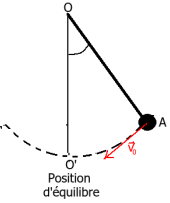
\includegraphics[width=0.18\textwidth]{./img/img02.png}
  \end{center}
\end{wrapfigure}
Un pendule est formé d’une tige rédige OA, de longueur l = 50cm, de masse négligeabl  et d’un corps ponctuel placé en A de masse m=200 g . On écarte le pendule d’un angle $\alpha$ = 30◦ par rapport à sa position d’équilibre stable et on le lance avec une vitesse initiale $\vec{V}$ orthogonale à la droite (OA) .

Les frottement sont négligeable . On prend l’état de référence pour l’énergie potentielle de pesanteur le plan horizontal qui passe par O’ et l’axe $O'z$ orienté vers le haut .

On donne g = 10N/kg

1. Déterminer la valeur minimale de $v_0$ pour que le pendule puisse effectue un tour complet.

2. Sachant qu’on le lance avec une vitesse $v_0 = 4, 5m/s$ , déterminer les valeurs minimales et maximales de la vitesse du corps et son énergie cinétique .

\end{Box2}

%%_________________________Exercice 4 : _________________________Exercice
\begin{Box2}{Exercice 4 : }
\begin{wrapfigure}{r}{0.39\textwidth}
  \begin{center}
    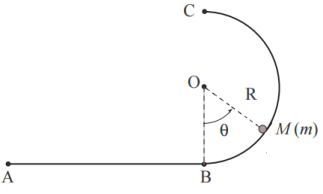
\includegraphics[width=0.37\textwidth]{./img/img03.png}
  \end{center}
\end{wrapfigure}
Un solide ponctuel de masse m est lancé en A sur une piste horizontale prolongée par un demi-cercle vertical de rayon R.
On donne : AB = 1 m ; R = 1 m ; m = 0, 5 kg ; g = 9, 81 N/kg

   1. Les frottements étant négligeables, calculer en A la vitesse minimale $V_{A_{min}}$ que doit avoir la masse pour qu’elle atteigne le point C

   2. Même question lorsque les frottements entre l’objet et la piste sont assimilables à une force constante de norme f=1N.

\end{Box2}

\vspace{2cm}
\begin{center}
   \Large{ \em{Exercices Supplémentaires}}
\end{center}



%%_________________________Exercice 5 : _________________________Exercice
\begin{Box2}{Exercice 5 : }
\begin{wrapfigure}{r}{0.39\textwidth}
  \begin{center}
    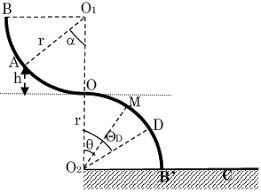
\includegraphics[width=0.37\textwidth]{./img/img04.png}
  \end{center}
\end{wrapfigure}
Une portion de gouttière BO de forme circulaire de rayon $r=1m$ se situe dans un plan
vertical. Elle se raccorde en O à une autre gouttière identique OB’ située dans le même plan (voir figure).

Les centres O1 et O2 des deux gouttières se trouvent sur la même verticale. Un solide ponctuel S de masse m=100g est lâché sans vitesse du point A situé à une hauteur h = 0,2 m par rapport au plan horizontal passant par O. Les frottements étant supposés négligeables et $g = 10kg/N$

1. En choisissant le point O comme origine des altitudes et comme position de référence, calculer l’énergie mécanique du solide.

2. Exprimer puis calculer la vitesse du solide VO au passage en O.

3. Sur le parcours OD le solide reste en contact avec la surface de la gouttière et sa position est repéré par l’angle $\theta = (\overrightarrow{O_2O}, \overrightarrow{O_2M})$
Etablir l’expression de la vitesse V du solide en un point M quelconque du trajet OD en fonction de h , r , g et $\theta$.

   4. Sur le trajet OD on montre que l’intensité R de la réaction de la gouttière sur S à pour expression $$R = mg(cos(\theta) - \frac{V^2}{r.g})$$
Au point D le solide S perd le contact avec la gouttière et suit le trajet DC. Déterminer la valeur numérique $\theta_D$ et celle de $V_D$ vitesse du S au point D.

   5. Avec quelle vitesse du solide touche-t-il le sol en C ?
\end{Box2}

\begin{Box2}{Exerice 6 : }
Un cycliste descend une pente de 10\% . Sa vitesse v = 54km/h est constante .

1. Calculer la variation de l’énergie potentielle de pesanteur pendant $\Delta$t = 1s .

2. Calculer la quantité de chaleur Q dissipée par les frottement au niveau des freins pendant 30s.

Donnée : L’ensemble cycliste -bicyclette a une masse m = 80kg L’intensité de pesanteur g = 9, 8N/kg

\end{Box2}

\begin{Box2}{Exerice 7 }
\begin{wrapfigure}{r}{0.39\textwidth}
  \begin{center}
    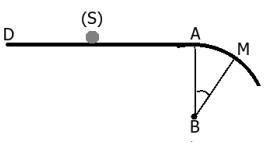
\includegraphics[width=0.37\textwidth]{./img/img05.png}
  \end{center}
\end{wrapfigure}

   Un skieur glisse sur une piste horizontale $DA$ à vitesse constante . En A, commence une portion de piste circulaire de rayon R =BA (B est à la verticale de de A ) . Les frottement sont négligeables et on admet que le skieur est assimilable à un point matériel dont la trajectoire suit la forme de la piste.

1. Calculer la variation de l’énergie mécanique enter le point A et le point M .

   2. Déduire l’expression de la vitesse de skieur au point M en fonction de R , $\theta=\Hat{ABM}$ et g
On prend g = 10N/kg

\end{Box2}
%%_________________________Exercice 6 : _________________________Exercice
\end{document}
